%%%%%%%%%%%%%%%%%%%%%%%%%%%%%%%%%%%%%%%%%
% Classicthesis-Styled CV
% LaTeX Template
% Version 1.0 (22/2/13)
%
% This template has been downloaded from:
% http://www.LaTeXTemplates.com
%
% Original author:
% Alessandro Plasmati
%
% License:
% CC BY-NC-SA 3.0 (http://creativecommons.org/licenses/by-nc-sa/3.0/)
%
%%%%%%%%%%%%%%%%%%%%%%%%%%%%%%%%%%%%%%%%%

%----------------------------------------------------------------------------------------
%	PACKAGES AND OTHER DOCUMENT CONFIGURATIONS
%----------------------------------------------------------------------------------------

\documentclass[10pt,a4paper]{scrartcl}

\reversemarginpar % Move the margin to the left of the page 

\newcommand{\MarginText}[1]{\marginpar{\raggedleft\itshape\small#1}} % New command defining the margin text style

\usepackage[dvipsnames]{xcolor}
\usepackage[nochapters]{classicthesis} % Use the classicthesis style for the style of the document
\usepackage[LabelsAligned]{currvita} % Use the currvita style for the layout of the document
\usepackage{graphicx}
\usepackage{caption}
\usepackage{wrapfig}
\usepackage[left=5cm,right=2.2cm,top=2cm,bottom=2cm]{geometry}

\hypersetup{pdftitle={CVCeciliaDiMauloEN},
    pdfauthor={Cecilia.DiMaulo},
    pdfsubject={},
    pdfkeywords={},
    colorlinks=false,       % no lik border color
    allbordercolors=white    % white border color for all
}

\definecolor{mediumtealblue}{rgb}{0.0, 0.33, 0.71}

\renewcommand{\cvheadingfont}{\LARGE\color{mediumtealblue}} % Font color of your name at the top


\usepackage{hyperref} % Required for adding links	and customizing them
\hypersetup{colorlinks, breaklinks, urlcolor=black, linkcolor=mediumtealblue} % Set link colors

\newlength{\datebox}\settowidth{\datebox}{10.2018-1.2018} % Set the width of the date box in each block

\newcommand{\NewEntryL}[3]{\noindent\hangindent=2em\hangafter=0 \parbox{\datebox}{\normalsize \textit{#1}}\hspace{5em} #2 #3 % Define a command for each new block - change spacing and font sizes here: #1 is the left margin, #2 is the italic date field and #3 is the position/employer/location field
\vspace{0.5em}} % Add some white space after each new entry

\newcommand{\NewEntry}[3]{\noindent\hangindent=2em\hangafter=0 \parbox{\datebox}{\normalsize \textit{#1}}\hfill\color{mediumtealblue}\spacedlowsmallcaps{#2} \color{black}#3 % Define a command for each new block - change spacing and font sizes here: #1 is the left margin, #2 is the italic date field and #3 is the position/employer/location field
\vspace{0.5em}} % Add some white space after each new entry

\newcommand{\Description}[1]{\hangindent=2em\hangafter=0\raggedright\footnotesize{#1}\par\normalsize\vspace{1em}} % Define a command for descriptions of each entry - change spacing and font sizes here

%----------------------------------------------------------------------------------------

\begin{document}

\thispagestyle{empty} % Stop the page count at the bottom of the first page

%----------------------------------------------------------------------------------------
%	NAME AND CONTACT INFORMATION SECTION
%----------------------------------------------------------------------------------------

\begin{wrapfigure}{L}{1em}
 \hspace*{-10em}
 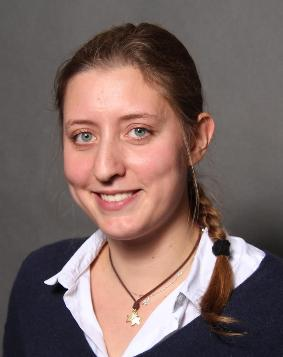
\includegraphics[scale=0.3]{img/ceci.jpg}
\end{wrapfigure}

\begin{cv}{\spacedallcaps{Cecilia Di Maulo} \ \ \ \ \ \ \  \color{black}\large\emph{25 years old}}\vspace{2em} % Your name

%\begin{wrapfigure}{License{1em}
% \hspace*{-10em}
% 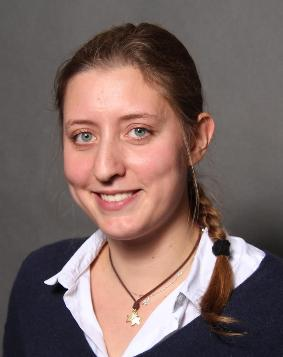
\includegraphics[scale=0.3]{img/ceci.jpg}
%\end{wrapfigure}

\NewEntryL{email}{\href{mailto:cecidimaulo@gmail.com}{cecidimaulo@gmail.com}} % Email address

\NewEntryL{phone}{ +33 6 26 30 86 90} % Phone number(s)

\NewEntryL{address}{ 4, rue du vieil abreuvoir, Saint-Germain-en-Laye, France} % Phone number(s)

\vspace{1.2em} % Extra white space betweelinksn the personal information section and goal

%\noindent\spacedlowsmallcaps{Goal}\vspace{1em} % Goal heading, could be used for a quotation or short profile instead

%\Description{Gain fundamental experience in my area of interest and expertise.}\vspace{2em} % Goal text

  \fcolorbox{white}{mediumtealblue}{\parbox{\dimexpr\textwidth-2\fboxsep-2\fboxrule}{\tiny\textcolor{white}{\hspace{1.5 cm}}}}

\vspace{1.5em} % Extra white space betweelinksn the personal information section and goal
%----------------------------------------------------------------------------------------
%	WORK EXPERIENCE
%----------------------------------------------------------------------------------------

  \noindent\color{mediumtealblue}\spacedallcaps{Work Experience}\vspace{1em}

  \color{black} \NewEntry{05.2018-...}{Cloud Computing Engineer}

  \Description{\MarginText{Osones}Mission: development of an offline OpenStack platform with a fully automated deployment
         \begin{itemize}
           \item {Ideation of the architecture (12 servers)} 
        \item {Evaluation and implementation of a baremetal deployment tool}
        \item {Evaluation and implementation of local mirrors}
        \item {Deployment automation: from server racking to an operational OpenStack}
        \end{itemize}
    \emph{Technologies: Ansible, OpenStack-Ansible, CentOS 7.O, Ironic, Git \& Gitlab}
 \newline 
  
  Mission at IRT SystemX: update of a production IaaS based on OpenStack
        \begin{itemize}
          \item {Upgrade of 4 versions of OpenStack (9 servers)} 
        \item {Integration of a service for additional volumes for the VMs}
        \item {Integration of a service of Load Balancing}
        \item {Integration of a service of metrology for the VMs}
        \end{itemize}
    \emph{Technologies: OpenStack-Ansible, Ubuntu 14.04 \& 16.04, Ansible, Terraform, iSCSI}
  }
%------------------------------------------------

  \NewEntry{10.2017-4.2018}{Cybersecurity research engineer}

  \Description{\MarginText{Thal\`{e}s Services}Evaluation of VNFs orchestration services    
        \begin{itemize}
          \item {Study and comparison of VNFs orchestration services}
          \item {Design of the architecture of an experimental 5G platform based on OpenStack}
        \end{itemize}
  }

%------------------------------------------------

\NewEntry{02-08.2017}{Master degree internship - research engineer}

\Description{\MarginText{Orange Labs Networks}Supervision of the 5G networks for IoT use cases}

%------------------------------------------------

\vspace{2em} % Extra space between major sections

%----------------------------------------------------------------------------------------
%	EDUCATION
%----------------------------------------------------------------------------------------

\color{mediumtealblue}\spacedallcaps{Education}\vspace{1em}


\color{black}
\NewEntry{2017}{Master Computer science for Communication Networks}

\Description{\MarginText{Universit\'e de Paris Saclay} 
\textbf{Master thesis} \textit{OSes for Cyber Physical Systems}, state of the art and performances study.}

%------------------------------------------------

\NewEntry{2014 - 2017}{Master Telecom engineer}

\Description{\MarginText{T\'el\'ecom SudParis, Evry}\textbf{First year project} with the start up Auticiel: "How to introduce tablets in nursing homes": \emph{Project management, Testing, Tutorial writing}\newline
    \textbf{First year programmation project}:
    "Mario-like game": \emph{C language (SDL), Tile-Mapping, Git}} 

%------------------------------------------------

\NewEntry{03-08.2016}{Exchange semester}

\Description{\MarginText{Universidade Federal do Ceara, Fortaleza, Brazil}\emph{Main courses: Software development for the cloud (AWS), Fuzzy Logic, Semantic Web, Artificial Intelligence, Portuguese}} 

%------------------------------------------------

\NewEntry{2011 - 2014}{Preparatory class to top level engineering schools}

\Description{\MarginText{Lyc\'ee Pasteur, Neuilly-sur-Seine}} 

%------------------------------------------------
\NewEntry{2011}{Scientific Baccalaur\'eat with international option}

\Description{\MarginText{Lyc\'ee International, St-Germain-en-Laye}\textbf{French and Italian Diploma} option Mathematics.} 

%------------------------------------------------
\vspace{22em} % Extra space between major sections

%----------------------------------------------------------------------------------------
%	OTHER INFORMATION
%----------------------------------------------------------------------------------------
\color{mediumtealblue}
\spacedallcaps{More Information}\vspace{1em}

\vspace{1em}

\color{black}
\newlength{\langbox} % Create a new length for the length of languages to keep them equally spaced
\settowidth{\langbox}{Francais} % Length equals the length of "English" - if you have a longer language in your list put it here

\Description{\MarginText{Languages}\parbox{\langbox}{\textsc{Italian}}\ \ $\cdotp$\ \ \ C2 - Mother Tong}

\vspace{-0.5em} % Negative vertical space to counteract the vertical space between every \Description command

\Description{\parbox{\langbox}{\textsc{French}}\ \ $\cdotp$\ \ \ C2 - Mother Tong}  

\vspace{-0.5em} % Negative vertical space to counteract the vertical space between every \Description command

\Description{\parbox{\langbox}{\textsc{English}}\ \ $\cdotp$\ \ \ C2}

\vspace{-0.5em} % Negative vertical space to counteract the vertical space between every \Description command

\Description{\parbox{\langbox}{\textsc{Portuguese}}\ \ $\cdotp$\ \ \ C1}

\vspace{1em} % Negative vertical space to counteract the vertical space between every \Description command

%------------------------------------------------

\Description{\MarginText{Hobbies}\textbf{Volley-ball} (level Nationale 3 for seasons 2009-2013),
    \textbf{Diving} (Rescue Diver Diploma),
    \textbf{Skiing} (9 downhill Giant, then 5 years freestyle skiing)
    \textbf{Passionate reader} (Italian, French and English classic litterature),
    \textbf{Traveling},
    \textbf{Piano and Saxophone}}
%----------------------------------------------------------------------------------------
\date{}
\end{cv}

\end{document}
